% Generated from 17-学术前沿技术专题.md; edit the LaTeX source after migration.

\reportpart{第十七部分 学术前沿技术专题}
\addcontentsline{toc}{part}{第十七部分 学术前沿技术专题}
\markboth{第十七部分 学术前沿技术专题}{第十七部分 学术前沿技术专题}

前面的章节已经建立了主干结构，本部分则集中讨论当前最值得跟踪的一批前沿问题。这些问题未必都已形成稳定产业路径，但它们最能暴露现代具身系统的真实能力边界，也最有可能在未来几年牵引模型、数据和本体设计的进一步分化。

本章的写法刻意不追求“热点罗列”，而更强调这些前沿方向各自卡在哪些瓶颈、为什么难、以及它们会反向推动哪些基础技术继续演化。很多真正有价值的前沿，不是因为它们最会讲故事，而是因为它们迫使研究者同时面对感知、接触、推理、控制和评测的多重困难。

\section*{80. 通用操作与灵巧操作}
\addcontentsline{toc}{chapter}{80. 通用操作与灵巧操作}
\markboth{80. 通用操作与灵巧操作}{80. 通用操作与灵巧操作}

\subsection*{80.1 通用抓取}
\addcontentsline{toc}{section}{80.1 通用抓取}


通用抓取之所以依旧是前沿专题，是因为它看起来像“基础能力”，实际上却牵动感知、几何、接触、控制与恢复的多层协同。系统若只能在已知物体、已知摆放和已知夹具条件下抓取，它解决的仍然是局部模板问题；只有当它能在对象变化、姿态变化和局部遮挡下保持稳定，抓取能力才开始接近更通用的操作入口。

因此，通用抓取不是一个已经做完的老问题，而是后续很多 VLA、触觉与世界模型路线是否真正落地的最低压测场之一。 通用抓取之所以长期是前沿主题，不是因为“抓东西”本身新，而是因为它要求系统在对象类别、材质、摆放方式、遮挡关系和接近路径都变化时，仍能形成稳定抓取。它同时考验感知、几何推理、接触控制和失败恢复，因此常被当作具身系统最基础也最顽固的能力基准之一。

通用抓取看起来是最基础的问题，但它至今仍是具身系统的重要瓶颈，因为对象多样性、遮挡、摩擦变化和接触不确定性始终存在。即便在基础模型时代，“看懂物体”也不等于“找到可执行抓取方式”。

通用抓取之所以仍然是前沿问题，并不是因为学界还没学会“把东西拿起来”，而是因为一旦对象库扩大、遮挡增加、材料变化、接触条件变化或任务上下文不同，抓取就会迅速从几何问题变成感知、接触和恢复共同参与的问题。也就是说，抓取是最基础的任务单元之一，但恰恰因为基础，几乎所有系统性短板都会在这里暴露。 这也是为什么通用抓取长期具有指标意义：谁能稳定提升抓取在长尾物体、复杂遮挡和失败恢复下的表现，谁就更可能真正改善具身系统的通用性，而不是只在少数干净场景里演示漂亮结果。

\subsection*{80.2 精细装配}
\addcontentsline{toc}{section}{80.2 精细装配}


精细装配之所以特殊，是因为它把误差容忍度压得极低。相比抓取和搬运，装配往往更依赖局部几何对准、接触过程感知、高频闭环修正和阶段性失败恢复。很多系统在非接触任务中看似稳定，一进入装配就会暴露出观察误差、控制滞后与接触建模不足。

因此，精细装配在研究中始终具有标杆意义。它不是为了展示炫技，而是在迫使系统回答“当误差预算极小、接触过程主导成败时，智能究竟如何组织”。 精细装配比通用抓取更进一步，因为它要求机器人在极小几何公差、复杂接触序列和高失败代价下稳定完成任务。这里的问题不只是“把对象抓起来”，而是“在接触中逐步逼近正确插入或装配状态”，因此对力觉、接触建模、局部搜索和异常恢复的要求都显著更高。

对学习者而言，可以把精细装配理解成“状态估计最困难、动作修正最频繁”的典型任务。视觉通常只能提供粗定位，真正决定成败的是接触后的微调阶段：是否感知到卡滞、是否识别插入方向偏差、是否知道该退回多少、重新接近时是否会重复犯同一种错误。这也是为什么精细装配常常比抓取更能暴露系统是否真的具备闭环接触智能。

精细装配要求系统不仅看懂目标，还要在毫米级甚至更精细尺度上稳定接触、定位和纠偏。这使它成为检验真实操作能力的硬指标。与粗粒度搬运不同，装配任务通常要求视觉、力觉与接触反馈持续协同。

精细装配之所以比粗粒度搬运更能检验真实能力，是因为它要求系统同时具备高精度位姿估计、接触时纠偏、力控稳定性与局部状态机恢复能力。插接、拧紧、卡扣和窄间隙对位这些任务，都会把“看起来懂任务”与“真的能执行任务”之间的差距迅速放大。 在研究上，装配任务因此非常珍贵，因为它把视觉、力觉、控制和动作表示这些在一般 benchmark 中容易分开的层面重新绑回同一条约束链上。一个系统若能在装配里稳定表现，它的含金量往往远高于在纯视觉 pick-and-place 场景中的高分。

\subsection*{80.3 双臂与多指协同}
\addcontentsline{toc}{section}{80.3 双臂与多指协同}


双臂与多指协同真正困难的，不是自由度简单增加，而是接触、约束和责任分工同时增加。一个末端执行器的误差可能立刻传递给另一只手，局部最优动作也更容易演化成全局冲突。因此，这类系统往往更依赖显式的阶段管理、接触状态估计和恢复逻辑，而不是单纯把单臂策略“复制两份”。谁能在这里维持跨执行器的一致状态与安全边界，谁才更接近可部署能力。 双臂与多指协同的难点，在于系统不再只是为单一末端执行器规划动作，而是要同时处理多个执行器之间的空间耦合、时序协调和力学相互影响。一个简单抓取动作，在双臂场景里可能涉及一只手固定、另一只手操作；在多指灵巧手中，则进一步涉及接触分布、指间力平衡和手内重抓（in-hand manipulation）。

一个最小协同控制抽象可以写成：

\begin{equation*}
a_t = \pi(o_t, x_t^{left}, x_t^{right}, c_t)
\end{equation*}

其中 \(c_t\) 表示双臂或多指之间的协调约束。对学习者来说，这一节最重要的是看到：这里的问题不是“自由度更多”这么简单，而是任务结构和接触结构都同步升级了。

双臂和多指协同把操作问题从单一抓取推进到协调时序、接触分配与力位协同，其难度远高于公开视频里看起来的“两个手一起动”。

更关键的是，这类任务会迫使系统显式处理“谁固定、谁操作、何时换手、何时局部重抓”这类中间策略问题。也就是说，双臂与多指协同不仅提高了控制难度，也提高了任务结构表达难度，因此经常成为检验高层规划与低层接触接口是否真正打通的压力测试。

\subsection*{80.4 为什么灵巧操作仍是“真能力试金石”}
\addcontentsline{toc}{section}{80.4 为什么灵巧操作仍是“真能力试金石”}


对学习者来说，灵巧操作最值得关注的并不是“炫技感”，而是它把许多平时被分开讨论的模块重新拧到了一起。一个灵巧操作系统通常必须同时回答：对象局部几何如何被感知、手指或夹爪如何建模接触、动作如何以足够高频率闭环修正、失败时如何局部重抓而不是整段重来。谁能在这个问题上给出自洽答案，谁的系统就更接近真实通用操作能力。 灵巧操作之所以仍是试金石，是因为它会同时放大感知误差、接触误差、控制误差和规划误差。很多系统在非接触、低精度、单步动作任务里看起来能力很强，但一进入多接触、细粒度、可恢复要求高的灵巧操作场景，真实上限就会迅速显现。

在很多公开系统里，最容易泛化的往往是接近抓放（pick-and-place）的结构化任务；而最能暴露能力上限的，通常是需要连续接触调节、局部纠偏和长期稳定性的灵巧任务。ACT、Diffusion Policy、灵巧手策略等路线之所以重要，就在于它们不断逼近这一难题，但还远未彻底解决，相关工作可参见 \href{https://arxiv.org/abs/2304.13705}{ACT} 与 \href{https://arxiv.org/abs/2303.04137}{Diffusion Policy}。

如果把灵巧操作进一步抽象，它其实是在逼迫系统同时优化三个目标：

\begingroup
\scriptsize
\begin{equation*}
\min_{\pi} \; \mathcal{L}_{\text{task}}
+ \lambda_1 \mathcal{L}_{\text{contact instability}}
+ \lambda_2 \mathcal{L}_{\text{regrasp cost}}
+ \lambda_3 \mathcal{L}_{\text{failure recovery delay}}
\end{equation*}
\endgroup

这里真正难的不是写出损失函数，而是这几个项在现实中往往没有稳定标签。接触不稳定常常只能通过力觉、滑移趋势或阶段性失败间接观察；重抓代价和恢复延迟则更多属于系统级指标，而不是单步动作标签。因此，灵巧操作之所以长期是“真能力试金石”，恰恰因为它让高层语义、局部接触、低层控制和系统恢复第一次被迫共同接受考核。

\section*{81. 可变形物体与复杂接触操作}
\addcontentsline{toc}{chapter}{81. 可变形物体与复杂接触操作}
\markboth{81. 可变形物体与复杂接触操作}{81. 可变形物体与复杂接触操作}

\subsection*{81.1 布料、绳索、软物体}
\addcontentsline{toc}{section}{81.1 布料、绳索、软物体}


布料、绳索和软物体任务值得持续关注，因为它们会迅速击穿很多刚体场景中仍可勉强成立的近似。对象状态高度部分可观、形变历史相关、接触结果难预测，这些特征都会迫使系统重新重视状态记忆、触觉反馈和更强的世界表征。

因此，这类任务并不只是更难的 manipulation benchmark，而是在系统性地逼问机器人：当对象的关键状态不再稳定显现在单帧视觉里时，你还能靠什么做决策。 这类对象之所以特殊，是因为它们没有稳定、低维、刚体式的状态描述。布料会折叠、绳索会缠绕、软物体会变形，导致“同一个任务目标”可能对应大量视觉上和接触上完全不同的中间状态。因此，这一方向天然更依赖触觉、世界建模和恢复策略。

这类对象会使状态表示、接触预测和任务规划极大复杂化，因此仍然是具身系统的难题高地。因为对可变形物体而言，“状态”本身就远比刚体复杂，很多时候既难感知，也难参数化。

布料、绳索、软物体这类对象之所以长期困难，是因为它们的“状态”本身就极难参数化。对刚体，系统还可以依赖位姿、几何和接触点近似；对可变形对象，这种近似会迅速失效，感知、预测与控制都需要面对高维形变空间。这意味着系统不仅难以决定该怎么做，甚至难以稳定描述当前世界到底处于什么状态。 因此，这类任务往往会反向推动表示学习、世界模型和触觉研究。因为只有当内部状态表示真正吸收了接触与形变结构，系统才可能在这类任务上形成可复用能力。

\subsection*{81.2 复杂接触建模}
\addcontentsline{toc}{section}{81.2 复杂接触建模}


复杂接触建模之所以始终是前沿难题，是因为许多真实操作任务的关键信息恰恰藏在最难建模的局部瞬间里。插接、装配、拧动、摩擦配合、材料形变和局部卡滞，都要求系统不仅知道“接触发生了”，还要理解接触如何演化、哪些力方向是安全的、哪些状态预示着即将失败。

如果把这类问题写成更抽象的形式，就是系统要在部分可观、强非线性和高噪声条件下估计隐藏接触状态 \(c_t\)，并据此调整动作：

\begingroup
\footnotesize
\begin{equation*}
\hat{c}_t = f(o_t, f_t, h_t), \qquad a_t = \pi(o_t, \hat{c}_t, g)
\end{equation*}
\endgroup

这里 \(o_t\) 可以是视觉与本体观测，\(f_t\) 可以是力/触觉信号，\(h_t\) 是近期历史。真正困难的不是写出这个式子，而是隐藏接触状态往往没有直接标签，且不同材料、不同装配公差、不同执行器柔顺性都会改变其观测分布。

对具身智能而言，这意味着复杂接触建模既不是纯物理问题，也不是纯感知问题，而是感知、控制、预测与本体顺应性共同交织的问题。很多路线最终都会被这类任务重新拉回到对身体与世界相互作用的细致建模上。 复杂接触建模的真正困难，不在于是否检测到“发生了接触”，而在于接触模式会连续切换：粘附、滑移、滚动、卡滞、局部变形、接触点迁移都可能在同一任务中出现。对布料、绳索和软物体来说，系统甚至很难定义一个稳定、低维、足够完备的状态。

复杂接触之所以长期难解，是因为它既不是纯感知问题，也不是纯控制问题。很多关键状态无法仅凭视觉稳定观测，而必须通过接触过程逐步显现；与此同时，接触结果又高度依赖瞬时力位关系和局部材料属性。

接触一旦从刚体碰撞扩展到滑移、卡滞、形变与摩擦不确定，系统就会迅速暴露感知和控制接口的脆弱性。机器人在布料整理、线缆操作、袋装物体处理和柔性装配中经常遇到这种情况。

\subsection*{81.3 评测难点}
\addcontentsline{toc}{section}{81.3 评测难点}


这类任务的评测之所以困难，是因为单一成功率往往不足以描述真实能力。系统可能最终完成了任务，但过程中过于依赖重试、局部碰撞、异常人工干预或极高节拍波动；也可能在标准件上成功，却在轻微尺寸变化或材料差异下立即失效。若评测口径过粗，就会高估系统真实可部署性。

因此，复杂接触与灵巧操作的评测更需要分层指标，例如成功率、恢复率、对扰动敏感性、节拍稳定性、对尺寸偏差的容忍度以及对感知/力觉缺失的退化表现。这些指标虽然更麻烦，却更接近真实能力边界。 这类任务的评测难点，首先在于成功标准本身就难定义。例如布料折叠是看边角对齐、皱褶程度还是最终可用性？绳索整理是看末端位置、结是否解开还是后续可操作性？这使得很多 benchmark 很难像刚体抓取那样用单一成功率概括。

评测难点还在于任务结果往往存在连续质量差异，而非简单二元成功失败。布料是否“足够平整”、线缆是否“可接受地整理”、装配是否“留有安全裕量”，都需要比单个成功率更细的度量体系。

复杂接触任务很难像标准分类 benchmark 那样有统一清晰指标，因此研究进展也更难横向比较。成功率之外，通常还需要记录纠偏次数、接触稳定性、操作时长和失败模式类型。

从研究方法上看，这一节最重要的启发是：只要评测仍然停留在粗糙成功率上，社区就会持续低估真实接触难度。越是接近复杂装配、柔性体操作和长期自主整理，越需要把恢复、节拍波动、局部错误传播和安全裕量显式写进评测指标。

\subsection*{81.4 为什么这类任务会推动世界模型与触觉路线继续前进}
\addcontentsline{toc}{section}{81.4 为什么这类任务会推动世界模型与触觉路线继续前进}


这也是为什么可变形物体任务对研究方向具有放大效应。它会把那些在刚体场景中还能被容忍的近似全部暴露出来，例如只靠视觉进行迟滞估计、只用末端位姿代表接触状态、只用成功率而不记录恢复代价等。某种意义上，这类任务就是在逼迫系统承认“环境的内部状态并不完全显现在图像里”，从而重新提升触觉、力觉和状态记忆的重要性。

这类高接触、高不确定性的任务之所以会持续推动世界模型与触觉路线前进，是因为单靠视觉和语言很难完整描述其中最关键的状态变量。对象内部受力、局部卡滞、柔性形变、滑移趋势和微小接触变化，常常只有在执行中才真正暴露出来。

因此，越是接近精细操作、装配、工具使用和柔性物体处理，系统就越需要某种能预测接触后果的内部模型，以及能感知细微接触差异的触觉通道。很多前沿路线看似分散，实则都在被这些真实任务约束重新拉回相似的问题核心。 原因很直接：仅靠远距离视觉往往不足以稳定恢复软物体的真实交互状态，而纯规则接触模型又难以覆盖其复杂变形。于是，研究自然会推动两条路线继续强化，一条是更能表达隐状态和未来演化的世界模型路线，另一条是更能直接观测接触状态的触觉路线。

可变形物体和复杂接触任务往往不能只依赖视觉前端，因为关键状态常常隐藏在接触内部。这使得世界模型若想真正服务于机器人，就必须吸收触觉、力觉和局部接触动力学；也迫使触觉路线从“附加模态”上升为部分任务中的核心模态。

一个更直观的理解方法，是把这类任务中的隐藏状态看作视觉无法完全恢复的潜变量 \(z_t\)：

\begin{equation*}
z_t = \phi(o_t, \tau_t, f_t, h_t)
\end{equation*}

其中 \(o_t\) 是视觉观测，\(\tau_t\) 是触觉/力觉读数，\(f_t\) 可以理解为局部接触特征，\(h_t\) 是历史信息。若模型只消费 \(o_t\)，它就会系统性低估那些真正决定任务成败、却不显现在图像里的接触信息。也因此，这类任务天然推动“多模态世界建模”从可选增强变成必要结构。

\section*{82. 人机协作与人类意图注入}
\addcontentsline{toc}{chapter}{82. 人机协作与人类意图注入}
\markboth{82. 人机协作与人类意图注入}{82. 人机协作与人类意图注入}

\subsection*{82.1 语言意图}
\addcontentsline{toc}{section}{82.1 语言意图}


人机协作中的语言意图理解，不只是把自然语言命令转成目标标签，而是要判断用户真正关心的目标、约束、容错和优先级。尤其在开放协作环境里，人类表达往往不完整、不精确，甚至会在执行过程中不断修正。因此系统需要的不只是语义解析能力，还需要交互式澄清和上下文记忆能力。

对具身系统而言，语言意图理解的价值在于降低人类编程门槛，但它只有在能稳定连接到任务结构和执行约束时才成立。 在人机协作场景里，语言意图的价值不只是让用户“更方便下命令”，而是让系统能够处理任务目标中的抽象约束、偏好表达和动态澄清。例如“先把危险的东西收起来”“顺手帮我把桌面也整理一下”这类要求，本身就带有模糊性与上下文依赖。

语言输入为机器人提供更自然的任务接口，但也把模糊性和歧义直接引入系统。

语言意图之所以构成前沿问题，不是因为“让机器人听懂一句话”本身有多新，而是因为自然语言天然带来语义压缩、模糊边界与上下文依赖。人类一句“把桌面整理一下”背后包含对象分组、优先级、可接受结果范围和环境约束，而这些通常并不显式给出。机器人若想真正利用语言，就必须把模糊任务要求映射为可执行子任务结构。 因此，语言意图研究真正难的地方并不是 ASR 或文本理解，而是语义到动作结构的落差填补。这也是语言在具身系统中长期不会只是一个“更方便的输入法”，而会持续牵引记忆、规划和技能接口设计。

\subsection*{82.2 示教与偏好}
\addcontentsline{toc}{section}{82.2 示教与偏好}


示教与偏好之所以值得单独讨论，是因为很多具身任务并不存在唯一标准动作序列。人类操作者之间往往只是在效率、安全、稳健性、保守程度或风格上存在偏好差异，而不是严格意义上的对错差异。若系统只能学习单一路径，它很可能在面对不同场景需求时显得僵硬。

把偏好信息引入训练，实质上是在让系统学习“什么样的成功更被接受”。这对具身系统尤其重要，因为现实部署中的可接受行为往往不只取决于任务是否完成，还取决于过程是否稳、是否易被人类理解、是否符合现场流程。 在人机协作专题里，示教与偏好之所以重要，是因为很多高质量协作行为无法只靠任务成功率定义。人类更关心的是机器人是否顺手、是否打断自己、是否动作可预期、是否需要频繁纠正。于是，人类示教提供“怎么做”，偏好反馈提供“哪种做法更符合协作习惯”。

这条路线的重要性，在于很多“做得更好”的标准并不容易由显式奖励函数刻画。例如人类可能偏好更稳的抓取路径、更少碰撞的搬运方式、更自然的整理顺序或更保守的接触策略。

示教、偏好反馈和纠偏记录是将人类隐性技能结构注入系统的主要路径。

如果把这个问题写成更明确的学习目标，可以把偏好信号看成在重写“成功”的排序而不仅是标签：

\begingroup
\scriptsize
\begin{equation*}
\pi^\star = \arg\max_{\pi}\; \mathbb{E}[R_{\text{task}}]
\lambda \, \mathbb{E}[R_{\text{human-pref}}]
\end{equation*}
\endgroup

这里 \(R_{\text{human-pref}}\) 可能对应更稳、更少打断、更可预期、或更符合现场流程的行为偏好。这个写法的重要意义在于，它说明偏好学习并不是主任务之外的装饰，而是在重写“什么样的成功值得被系统长期重复”。

近年的工作已经把这一点做得更具体。例如，\href{https://arxiv.org/abs/2606.03949}{arXiv:2606.03949} 不再只把人类反馈当成结果排序，而是把人类干预触发的信息重新用于 credit assignment；\href{https://arxiv.org/abs/2606.32027}{arXiv:2606.32027} 则进一步允许用自然语言定义速度、谨慎程度、稳定性等偏好轴，说明偏好学习正在从“二元选优”走向“多维行为风格约束”。这意味着示教与偏好正在逐渐形成一条连续接口：示教告诉系统“可行解在哪里”，偏好告诉系统“哪类可行解更值得保留”。

\subsection*{82.3 共融控制与共享自治}
\addcontentsline{toc}{section}{82.3 共融控制与共享自治}


共融控制与共享自治的重要性，在于它们把“人和系统如何共同完成任务”从过渡方案变成了研究对象本身。许多高价值场景并不要求系统一开始就全自主，而是要求它在关键片段自主、在高风险时可接管、在不确定时可请求人类输入。

这类研究路线的价值，恰恰在于它们更贴近现实组织方式。共享自治若能被设计成稳定接口，而不是临时兜底手段，那么很多原本被视为“还不够自主”的系统，反而可能更早形成商业价值。 共融控制与共享自治关注的是：人和机器人不是简单轮流接管，而是共同参与同一控制闭环。系统需要决定哪些变量由人主导，哪些变量由机器人主导，以及何时在两者之间动态切换。它不是纯自动，也不是纯遥操作，而是中间大量现实可落地场景的重要组织形式。

从研究角度看，共享自治不是“自动化不够强时的临时方案”，而是一种长期系统设计范式。它要求系统明确划分哪些决策适合自动执行、哪些节点应保留给人类确认、以及在异常时如何平滑接管与退出。

shared autonomy 的重要性越来越明显，因为很多高价值任务并不适合也不需要完全自动化。

把共享自治写成最小形式，可以表示为：

\begingroup
\scriptsize
\begin{equation*}
u_t = \alpha_t u_t^{\text{human}} + (1-\alpha_t)u_t^{\text{robot}}, \qquad
\alpha_t \in [0,1]
\end{equation*}
\endgroup

真正困难的地方并不在这个线性写法本身，而在于 \(\alpha_t\) 绝不能只是经验常数。它必须取决于任务阶段、环境风险、模型不确定性、人类负荷以及当前交互契约。也就是说，共享自治研究本质上是在研究“控制权如何流动”，而不是简单研究“谁更强”。

这一点在经典 shared autonomy 文献里就已经存在。\href{https://arxiv.org/abs/1701.07851}{arXiv:1701.07851} 强调的是系统既要推断人类目标，也要适应人类对系统的信任与可接受性；而更新的 \href{https://arxiv.org/abs/2506.16044}{arXiv:2506.16044} 则明确把人类意图建模、控制混合、责任边界与伦理问题放回统一框架里。再往前一步，\href{https://arxiv.org/abs/2503.07771}{RoboCopilot} 这类工作说明“示教 - 自主 - 再纠偏”可以不是三段式孤立流程，而是一条连续切换的人机共融学习链。

因此，共享自治之所以值得长期保留在主线里，不是因为它替完全自主“补短板”，而是因为它更真实地反映了很多高价值任务的组织方式：系统并不需要每一秒都赢过人类，而需要在关键片段里比“人独做”更稳、比“机独做”更可审计。

\subsection*{82.4 人类为什么不会很快退出回路}
\addcontentsline{toc}{section}{82.4 人类为什么不会很快退出回路}


所以更现实的目标，不是幻想“彻底去人化”，而是持续优化人类在回路中的位置。好的系统会让人类逐渐从低价值的机械接管中退出，转向高价值的目标设定、风险确认和异常仲裁；差的系统则会把人一直钉在高强度、低透明度的补锅位置上。这种区别会直接决定一个系统是否真的具备组织层面的可扩展性。

人类不会很快退出回路，并不是因为系统永远达不到更高自主性，而是因为在许多高价值场景里，人类本身承担的并不只是动作执行，还包括责任承担、异常裁决、流程协调、偏好表达和跨任务切换判断。这些职责很难在短期内被单一模型完整替代。

因此，很多现实系统真正演化的方向，并不是“迅速去人”，而是把人的角色从高频直接操作转移到监督、纠错、授权和边界条件处理上。谁能更好地设计这层协作接口，谁往往更接近真实落地。 人类短期内不会退出回路，根本原因不只是模型还不够强，而是现实场景中存在大量责任、偏好、异常判断和价值权衡，不适合完全交给自主系统一次性决定。越是开放、非结构化、责任高的场景，这一点越明显。

从系统设计角度看，这意味着“人在回路”不应被理解为临时补丁，而应被视为长期存在的架构假设之一。很多真正可落地的人机协作系统，反而正是因为认真设计了人类何时介入、如何介入、介入后如何回到自动流程，才具备现实价值。

从工业、医疗到危险环境，很多真实任务更现实的目标并不是“完全替代人”，而是“让人类把注意力集中在高价值决策点”。这意味着人机协作研究并不是通用自主的过渡形态，而很可能是长期稳定存在的主线。

从系统组织角度看，人类长期留在回路中的原因还可以写成一个职责再分配问题。随着模型能力提升，人类不会简单消失，而更可能从“连续操作者”转成“目标设定者、异常仲裁者和责任承担者”。若系统只能把人从高频操作位移到高频补锅位，那么它并没有真正降低组织负担；只有当系统把人稳定推向低频高价值决策位时，shared autonomy 才真正成立。这也是后续分析所有人机协作路线时最该追问的判据。

若把这一点写成更可操作的判断标准，可以直接追问三件事：人类是否仍被迫高频盯屏，系统是否能在交接前提供足够上下文，人类介入后是否能稳定回到自动流程。只有这三件事同时成立，“人在回路”才意味着组织效率提升；若其中任意一项长期失灵，那么人在回路就仍然更接近隐藏式人工补锅，而不是真正成熟的 shared autonomy。

\section*{83. 端侧与小模型路线}
\addcontentsline{toc}{chapter}{83. 端侧与小模型路线}
\markboth{83. 端侧与小模型路线}{83. 端侧与小模型路线}

\subsection*{83.1 on-device VLA}
\addcontentsline{toc}{section}{83.1 on-device VLA}


On-device VLA 之所以成为前沿议题，是因为它直接检验大模型路线能否脱离高算力实验条件，进入低时延、低功耗、弱联网的真实部署环境。若 VLA 只能依赖远程推理和大规模云算力，它的适用场景会被大幅收窄；一旦它能在端侧运行，很多移动平台、消费级和边缘场景的可能性才会真正打开。

因此，on-device 不是“缩小版大模型”这么简单，而是重新平衡语义能力、模型结构、压缩策略、异步推理与本地控制职责的系统工程问题。

端侧路线的重要性在于，它更接近真实部署的时延、隐私和功耗约束。近期无论是 DeepMind 的 Gemini Robotics 路线，还是 Figure 的 Helix 机载双系统结构，都在强调“能部署”本身已经成为研究目标，而不是最终再考虑的工程细节。 更轻量化的 SmolVLA 则进一步说明，部署约束已经开始反过来塑造模型设计目标。 相关资料可参见 \href{https://deepmind.google/blog/gemini-robotics-brings-ai-into-the-physical-world/}{Gemini Robotics 官方介绍}、\href{https://www.figure.ai/news/helix}{Figure Helix 官方介绍} 与 \href{https://arxiv.org/abs/2506.01844}{SmolVLA 论文}。

on-device VLA 的研究意义，在于它强迫学界把“是否能部署”提前成研究问题，而不是最后的工程善后。端侧算力、显存、功耗和散热会反过来约束模型结构、推理频率与动作接口，因此端侧路线不是大模型路线的低配复制，而是另一套目标函数下的重新设计。 也正因为如此，端侧研究常常会倒逼高低频分层、模型蒸馏、局部记忆外置和技能层重建等思路发展。谁如果忽视这一点，就会把端侧研究误看成单纯压缩问题。

从目前公开的一手材料看，端侧路线已经不再只是概念验证。Google DeepMind 在 \href{https://deepmind.google/blog/gemini-robotics-on-device-brings-ai-to-local-robotic-devices/}{端侧版本官方说明} 中明确把“本地低时延推理、脱离数据网络运行、少量示教快速适配”作为产品化能力来描述，并给出“约 50 到 100 条示教即可适配新任务”的工程口径；Figure 在 \href{https://www.figure.ai/news/helix}{Helix 官方介绍} 中则更进一步公开了异步双系统设计：高层视觉-语言模型 \texttt{\detokenize{S2}} 以 \texttt{\detokenize{7-9 Hz}} 运行，低层视觉运动策略 \texttt{\detokenize{S1}} 以 \texttt{\detokenize{200 Hz}} 运行，并部署在双嵌入式 GPU 上。它们共同说明，端侧具身模型真正被考验的，不是“能不能跑通一次前向”，而是“能否在物理控制时钟内稳定承担自己的责任层”。

如果把这类系统写成最小时间预算约束，可以表示为：

\begingroup
\scriptsize
\begin{equation*}
T_{\text{high-level infer}} < \Delta t_{\text{subgoal}}, \qquad
T_{\text{low-level loop}} < \Delta t_{\text{servo}}
\end{equation*}
\endgroup

前一个不等式约束高层语义规划是否来得及更新子目标，后一个不等式约束低层控制是否仍能维持姿态、接触和轨迹稳定。这个形式之所以重要，是因为它说明端侧 VLA 的关键并不只是“模型小型化”，而是“按频率域重新划分责任”。只要高层与低层的时间预算没有被明确写清，所谓 on-device 进展就很容易停留在演示叙事而不是系统能力。

\subsection*{83.2 小模型蒸馏与压缩}
\addcontentsline{toc}{section}{83.2 小模型蒸馏与压缩}


小模型蒸馏与压缩的核心目标，不只是把参数量变小，而是尽量保留大模型在任务理解或动作生成上的关键结构，同时把推理成本压到端侧可接受范围。常见路线包括知识蒸馏、量化、剪枝、低秩适配和动作头轻量化。

一个极简蒸馏流程可以写成：

\begin{lstlisting}[language=python]
teacher_actions = teacher(context)
student_loss = distill(student(context), teacher_actions)
update(student, student_loss)
\end{lstlisting}

小模型路线真正困难的地方，不在于把大模型“做小”，而在于决定哪些能力必须保留、哪些能力可以外包给检索、技能层或外部记忆。若只是机械压缩，往往最先损失的恰恰是长尾恢复与跨任务迁移能力。

若基础模型永远只能在超大算力上运行，其应用边界会被极大限制，因此蒸馏、量化和模块化裁剪会长期重要。这里的目标不只是压缩参数量，而是寻找在任务结构上真正必要的模型部分。 进一步说，蒸馏对象本身就需要分层。对具身系统而言，至少可以蒸馏三类东西：语义决策分布、动作生成分布，以及异常恢复偏好。前两者决定学生模型能否在常规轨道上复现教师模型，第三类则决定学生模型在长尾情境下会不会迅速坍塌。很多“压缩后平均分还行”的模型，一旦进入真实部署就显得明显脆弱，原因往往不是常规动作不会做，而是恢复动作、保守策略和停止条件没有被一并蒸馏下来。 因此，更合理的蒸馏评估不应只看主任务成功率，还应看延迟、功耗、异常恢复率和安全退化方式。一个更小的模型如果显著降低了推理时延，却也显著放大了错误自信或误触发频率，那么它未必真的比大模型更适合端侧。对后续产业判断而言，这一点尤其重要，因为不少“端侧能力突破”真正有价值的地方，不在于参数压缩本身，而在于团队是否找到了保留关键行为结构、同时接受部分语义损失的系统折中点。

把这个目标写成更接近系统设计的形式，可以表示为：

\begingroup
\scriptsize
\begin{equation*}
\mathcal{L}_{\text{student}}
= \mathcal{L}_{\text{task}}
 \alpha\, D_{\mathrm{KL}}(\pi_T \,\|\, \pi_S)
 \beta\, \mathcal{L}_{\text{latency}}
 \gamma\, \mathcal{L}_{\text{safety-regret}}
\end{equation*}
\endgroup

其中 \(D_{\mathrm{KL}}(\pi_T \,\|\, \pi_S)\) 不是为了机械逼近教师模型，而是为了尽量继承教师在动作分布、恢复偏好和保守边界上的结构；\(\mathcal{L}_{\text{latency}}\) 与 \(\mathcal{L}_{\text{safety-regret}}\) 则把端侧部署的真实代价显式拉回训练目标。也正因为如此，近年的轻量化路线越来越不是单纯量化或剪枝，而是与动作表示、分层架构和运行时一起共同设计，例如 \href{https://arxiv.org/abs/2506.01844}{SmolVLA} 与 \href{https://github.com/huggingface/lerobot}{LeRobot} 这类社区路线，实际上都把“模型能力”与“低门槛真实部署”并列成了目标，而不是先追最大模型、再在后处理中被动压缩。

这一节最容易被误读的地方，是把“压缩后还能做任务”误认为“压缩后仍保留了同样的系统价值”。对具身系统而言，真正珍贵的往往不是常规轨道上的平均动作，而是长尾失败时的保守动作、恢复动作和停机条件。因此，轻量化路线必须明确回答：它保留的是语义理解、动作分布、异常偏好，还是只是保留了一个在干净场景里还能跑通的平均政策。若这个问题不被显式回答，小模型路线就很容易只在演示里成立，而在现场运维时迅速露出脆弱性。

\subsection*{83.3 低成本机器人平台上的部署尝试}
\addcontentsline{toc}{section}{83.3 低成本机器人平台上的部署尝试}


低成本平台部署尝试的重要性，在于它们迫使研究路线面对更现实的资源约束。算力不足、传感器受限、执行器精度不高、结构余量有限，这些条件会暴露哪些方法只是依赖高配置堆出来的结果，哪些方法在更朴素平台上仍然保留核心价值。

从长期看，这类尝试不只是“便宜版验证”，而是对可扩散性的压力测试。很多路线若只能在高昂平台上成立，其产业外溢速度和规模化潜力就会受到显著限制。 低成本平台部署尝试的价值，在于它逼迫研究者正视“少算力、差传感、低精度执行器、简化夹爪和脆弱通信”这些通常被高端平台掩盖的问题。很多方法只有在这种平台上跑过，才真正知道哪些能力是算法本体带来的，哪些其实依赖昂贵硬件兜底。

这类尝试的意义，还在于它迫使研究者面对真实资源约束下的接口重构问题。廉价平台常常意味着更低控制频率、更差传感器、更少算力和更松机械精度，因此任何仍能保持可用性的系统，通常都在结构上做出了更强的工程折中。

低成本平台是检验具身路线是否具备扩散潜力的重要试验场。因为只有在廉价平台上仍能维持足够能力，某条技术路线才更可能被社区广泛复现和继续迭代。

这也是为什么“低成本平台”不应只被理解为教学玩具。Google DeepMind 在 \href{https://deepmind.google/blog/gemini-robotics-on-device-brings-ai-to-local-robotic-devices/}{端侧版本官方说明} 中明确展示了同一本地化基座模型从 ALOHA 双臂平台继续适配到 Franka FR3 与 Apptronik Apollo 的路线；\href{https://github.com/huggingface/lerobot}{LeRobot 开源项目} 则把“从低成本机械臂 \texttt{\detokenize{SO-100}} 到人形平台的硬件无关接口”与统一数据格式、统一评测脚本放在同一工具链里。前者说明“轻平台”正在被主流基础模型团队当作适配压力测试，后者说明社区侧也开始把“廉价可复现平台”视作开源生态真正扩散的必要条件。

从研究方法上说，低成本部署尝试最有价值的地方在于它能帮助我们区分三种能力：第一种是高端硬件直接兜底出来的能力；第二种是算法在控制频率下降、传感噪声升高后仍能保留的能力；第三种是依靠更好接口切分而不是更高配置硬件获得的能力。只有第二种和第三种，才更接近可扩散的系统资产。也因此，本节后续维护时，最值得记录的不是“某个便宜平台也跑通了”，而是“它删掉了哪些硬件奢侈项后，系统仍然保住了哪些能力”。

\subsection*{83.4 异步推理与高低频分层的新价值}
\addcontentsline{toc}{section}{83.4 异步推理与高低频分层的新价值}


异步推理与高低频分层之所以重新重要，是因为端侧部署常常无法让最强模型以控制频率持续前向。于是系统会重新采用“低频高语义模型 + 高频低层控制器”的架构，让大模型负责阶段决策，小模型或解析控制器负责局部闭环。

这一思路的真正价值，不只是“算力不够时的妥协”，而是帮助系统显式地区分哪些决策必须高语义、哪些决策必须高带宽。环境理解、任务改写、策略切换和异常归因通常不需要毫秒级更新，却需要更强的抽象能力；接触稳定、轨迹跟踪、阻抗调节和快速避障则恰恰相反。把两者硬塞进同一频率、同一模型，不但成本高，还容易让系统在关键环节上两头不到岸。

异步架构还要求一个容易被忽略的设计点：何时允许慢通路打断快通路。若高层模型的输出更新没有清晰触发条件，系统就可能在执行过程中频繁被新语义建议打断，表现为动作抖动、策略摇摆或安全边界失稳。更成熟的做法，是把高层推理的介入条件显式化，例如只在阶段完成、观测分布显著偏移、任务失败或人类指令变化时触发重解释。这样高低频分层才不是简单的“两个模型叠在一起”，而是真正经过接口治理的系统结构。

这一趋势说明，很多前沿工作真正回到的是“如何组织不同频率智能”而不是“如何让一个模型包打一切”。在资源受限平台上，异步推理不是妥协，而可能是更合理的系统最优：把昂贵推理只用在高价值阶段，把高频稳定性交给更轻、更确定的模块。

这条路线的新价值在于，它不是对大模型能力的否定，而是把模型能力重新放回受物理时钟和算力预算约束的真实系统里。对前沿研究而言，这恰恰可能是从“演示成功”走向“持续可运行”的关键一步。

轻量部署并不一定意味着“模型越小越好”。很多时候，更有效的办法是把高频控制和低频语义推理拆开：高层慢思考、低层快反应、异步通信。这使得大小脑分层不只是理论选择，也成为现实的端侧部署优化策略。

如果把异步推理写成更可执行的调度规则，可以理解为：

\begin{lstlisting}
仅当阶段完成 / 观测分布突变 / 人类目标改变 / 失败触发时，
才允许慢通路重解释并改写当前高层子目标；
否则快通路持续跟踪当前局部目标。
\end{lstlisting}

这个规则之所以重要，是因为许多系统失败并不是“高层模型不够强”，而是高层建议过于频繁地打断快通路，导致动作抖动、策略摇摆和安全边界失稳。异步分层真正成熟的标志，不是两个频率域都存在，而是慢通路何时有权改写快通路被说清楚了。

因此，端侧研究的真正价值并不只是压缩参数，而是重新设计能力分工：哪些能力必须留在端侧高频运行，哪些能力可以低频异步调用，哪些能力适合外包给检索、技能库或人类监督。谁能把这组分工做清楚，谁就更可能把“能跑”推进成“能长期稳定运行”。

如果把这类系统写成最小运行框架，它通常更像这样：

\begin{lstlisting}[language=python]
while robot_alive:
    low_level_state = controller.read()
    controller.stabilize(low_level_state)

    if planner_clock.tick():
        high_level_ctx = memory.pack_context()
        subgoal = vlm_planner.infer(high_level_ctx)
        controller.update_subgoal(subgoal)
\end{lstlisting}

这段伪代码的价值在于把一个经常被宏大叙事掩盖的现实说清楚了：很多端侧路线真正优化的，不是“让一个模型包打一切”，而是“如何让不同频率、不同责任层的智能模块在同一系统里稳定共存”。这也是为什么端侧与轻量路线并不只是压缩问题，而是架构重组问题。

如果结合当前公开系统看，这种架构重组已经是事实而不是建议。\href{https://www.figure.ai/news/helix}{Helix 官方介绍} 把高层语义理解与低层 \texttt{\detokenize{200 Hz}} 反应控制明确拆开，并让高层异步更新潜变量而不是直接逐控制步覆盖动作；\href{https://deepmind.google/blog/gemini-robotics-on-device-brings-ai-to-local-robotic-devices/}{端侧版本官方说明} 则进一步强调本地低时延与低层安全控制器共存。两者其实在回答同一个问题：高层模型应当在什么频率、以什么形式影响控制栈，才既不浪费语义能力，也不破坏物理稳定性。

这也是为什么我更倾向把异步推理理解为“职责治理”而不是“系统技巧”。一旦系统明确了高层只负责子目标、解释与阶段切换，低层负责接触稳定、约束满足与快速回退，那么后续无论替换更强模型还是更小模型，系统都更容易演化。反过来，若责任边界没有被写清，模型越强、系统越复杂，失稳的来源反而越难定位。

\section*{84. 持续自主与自我改进}
\addcontentsline{toc}{chapter}{84. 持续自主与自我改进}
\markboth{84. 持续自主与自我改进}{84. 持续自主与自我改进}

\subsection*{84.1 长时程任务执行}
\addcontentsline{toc}{section}{84.1 长时程任务执行}


长时程任务的根本难点在于系统必须维持“任务进行到了哪里”这一中间事实的连续可靠性。只要阶段状态、对象历史或资源占用信息在长链路中逐渐失真，后面每一步看似合理的局部动作都可能建立在错误前提上。因此，长时程能力的核心不只是更长上下文，而是更稳的任务状态机、更强的中途重规划和更清晰的失败分层恢复机制。 长时程任务执行的难点，不在于单步动作是否正确，而在于系统能否在较长时间里维护任务状态、子目标顺序、对象历史、失败恢复和资源占用信息。它要求的不只是更长上下文窗口，而是更强的任务记忆、状态管理和中途重规划能力。

长时程自主真正难的不是“序列更长”，而是状态漂移、环境变化、失败恢复和记忆管理同时变难。

长时程任务执行的真正困难，并不只是“序列更长”，而是系统必须在更长的时间轴上管理状态漂移、记忆衰减、异常恢复和环境变化。很多模型在短程任务上看似稳定，但一旦执行时间被拉长，局部小误差就会积累成结构性失效。 因此，长时程自主更像是对整套系统架构的考验，而不只是对某个策略模型的考验。记忆、重规划、恢复、监控和人类接管接口都会在这一层重新变得关键。

若把长时程执行写成形式化问题，可以把系统内部任务状态写成一个随执行演化的隐变量 \(m_t\)：

\begingroup
\footnotesize
\begin{equation*}
m_{t+1} = F(m_t, o_t, a_t, e_t), \qquad
a_t = \pi(o_t, m_t, g)
\end{equation*}
\endgroup

其中 \(m_t\) 不只是“上下文缓存”，还包含阶段进度、对象历史、资源占用、失败计数与局部异常标签；\(e_t\) 则代表环境突变或外部事件。很多模型在短任务上表现良好，却在长任务里持续退化，根源常常不是单步动作不会做，而是 \(m_t\) 在执行中逐渐失真，导致高层后续每次决策都建立在越来越不可信的任务事实之上。这个视角能帮助我们把“长时程能力不足”重新诊断为状态管理、重规划与恢复接口问题，而不是笼统归咎于上下文窗口不够长。

\subsection*{84.2 自主探索}
\addcontentsline{toc}{section}{84.2 自主探索}


自主探索在机器人里始终重要，因为很多关键能力无法仅靠离线示教覆盖完全。系统必须在可控风险下主动接触新状态、新对象和新场景，才能持续扩展能力边界。但机器人探索与纯软件探索不同，它的每一步都伴随物理成本、设备磨损和安全风险。

因此，真正值得关注的不是“是否自主探索”，而是探索如何被约束、如何被记录、以及如何与后续数据闭环衔接。谁能把探索组织成低风险高信息增益的过程，谁就更有机会在长期迭代中占优。

自主探索在具身系统里远比纯仿真强化学习更复杂，因为系统的每一次试探动作都带着真实成本：时间、能耗、磨损、风险以及对周边环境的潜在影响。这意味着现实中的探索不能只追求信息增益最大化，还必须同时考虑安全和可恢复性。

因此，真实机器人里的探索更像“受约束试探”而不是“自由试错”。一个更合理的目标往往不是最大化新颖性，而是在风险预算内优先探索那些最有可能缩小任务不确定性的动作片段。也正因为如此，持续自主若想真正成立，探索策略必须与回退策略、异常记录和数据回流基础设施一起设计，而不能被当作独立算法外挂。

因此，真正有价值的自主探索研究，往往不是鼓励机器人“多试几次”，而是研究如何在安全约束下高效选择最值得试的动作，如何把少量高价值探索与人类示教、世界模型和先验知识结合起来。 持续自主系统中的自主探索，并不是让机器人无约束“自己试一切”，而是在安全边界内主动寻找最能提升模型能力的新样本或新情境。对具身系统而言，真正有价值的探索通常是受约束的：去补当前最不确定、最常失败、最影响部署价值的区域，而不是平均地乱试。

对机器人而言，自主探索最大的障碍不是“不会探索”，而是探索成本太高且出错代价太大。每一次真实碰撞、跌倒、夹持失败或环境扰动都可能带来硬件损耗与安全风险，因此探索策略必须天然带着约束、审计和可回滚机制。

自主探索对具身系统很有吸引力，但在现实中始终受样本效率和安全边界限制。

若把真实探索目标写得更像具身系统问题，而不是纯强化学习问题，它更接近：

\begingroup
\scriptsize
\begin{equation*}
a_t^\star = \arg\max_a \; \text{InfoGain}(a \mid s_t)
- \beta \, \text{Risk}(a \mid s_t)
- \gamma \, \text{Wear}(a)
\end{equation*}
\endgroup

其中 \texttt{\detokenize{Risk}} 对应跌倒、碰撞、异常接触、环境损害等风险，\texttt{\detokenize{Wear}} 对应真实硬件磨损与维护代价。这个表达式的价值在于，它把“探索”重新拉回现实机器人的物理账本: 不是任何新样本都值得拿，而是要在风险预算里选最值得试的样本。

也正因此，长时自主文献经常最终回到“探索如何被约束与审计”。例如，\href{https://arxiv.org/abs/2212.12798}{arXiv:2212.12798} 强调的就不是抽象探索最优性，而是在线适应、环境变化与板载资源约束如何共同塑造长期自主。这种口径与本报告的判断是一致的：探索不是独立子算法，而是持续自主基础设施的一部分。

\subsection*{84.3 自动数据回流与自我修正}
\addcontentsline{toc}{section}{84.3 自动数据回流与自我修正}


这一方向之所以值得高度关注，是因为它把“部署后还能否继续变强”从模型问题提升为组织问题。什么片段值得回流、谁来标注、如何避免噪声放大、更新后如何回归验证，决定了系统会形成正反馈还是负反馈。很多团队并不缺模型更新能力，真正缺的是把失败日志稳定转写为高价值训练样本的流水线能力。这也是持续自主最终会回到数据治理、审计和版本回归基础设施的原因。 自动数据回流与自我修正的目标，是让系统在部署中遇到新失败模式后，不必完全依赖人工手工整理样本，而能自动记录关键片段、打上事件标签、进入再训练或再评测流程。它对应的不是单个算法，而是一整条“运行中发现问题 -> 形成样本 -> 进入训练闭环”的基础设施能力。

自动回流之所以是前沿问题，是因为它要求系统具备判断“什么值得回流、如何重标注、何时允许更新”的元能力。若所有日志都无差别回灌，训练会被噪声与重复样本淹没；若筛选过严，系统又会错过最有价值的长尾异常片段。

真正可持续的学习系统，需要把部署中遇到的新条件转回训练闭环，这也是未来系统是否会逐渐“越用越强”的关键。

更实用的写法，是把回流看成一个有损采样问题，而不是“尽量保存更多日志”：

\begingroup
\scriptsize
\begin{equation*}
\mathcal{D}_{\text{return}} =
\operatorname{Select}\!\bigl(\mathcal{L}_{\text{runtime}},\;
\text{novelty},\;
\text{failure severity},\;
\text{recoverability},\;
\text{annotation cost}\bigr)
\end{equation*}
\endgroup

这个式子背后的意思很朴素：不是所有运行日志都值得进入再训练集，真正高价值的片段通常同时满足“新”“重要”“可解释”“可被标注并回归验证”。也因此，持续自主路线最终一定会回到事件检测、异常分级、版本回归和灰度发布体系，而不会只停留在“自动把数据再喂回模型”这种抽象叙述上。对具身系统来说，若没有这一层选择与审计机制，自我改进极容易退化为自我污染。

近年的工作已经开始把这条链条显式系统化。例如，\href{https://arxiv.org/abs/2509.23829}{arXiv:2509.23829} 把示教、残差强化学习、滚动执行和数据增广组织成飞轮；\href{https://arxiv.org/abs/2603.11811}{arXiv:2603.11811} 则把语义规划、自动成功评估、环境自动复位和数据路由接起来，说明“自动回流”真正难的不是存日志，而是把运行事件可靠地翻译成高价值训练样本；\href{https://arxiv.org/abs/2511.19647}{arXiv:2511.19647} 更进一步强调部署机器人本身就是数据引擎，而不是训练结束后的静态执行器。三者共同说明：持续自主的关键不在“会不会继续采集数据”，而在“部署、筛选、标注、适配、回放”能否被真正闭环化。

\subsection*{84.4 持续自主的真正门槛}
\addcontentsline{toc}{section}{84.4 持续自主的真正门槛}


从这一角度看，持续自主的门槛本质上并不只在算法，而在系统是否拥有稳定的自我修正基础设施。没有结构化失败记录，就无法知道该回流什么数据；没有版本化回归测试，就无法判断新模型是在变强还是在引入新风险；没有局部恢复机制，系统就会在长时程任务里频繁因为小错中断。真正的“长期自主”因此更像一套长期运营能力，而不是一个单点模型突破。

如果把持续自主简单理解成“模型能连续运行更久”，就会低估问题难度。真正困难的地方在于，系统需要在长时间运行中持续吸收噪声、局部错误、硬件漂移和任务变化，而不是只在理想条件下延长单次成功轨迹。也正因此，持续自主的门槛往往体现在日志系统、回放工具、异常分级、在线监测、灰度发布和数据回流策略这些看似不够“学术前沿”的基础设施上。

从研究到产品的跨越，也常在这里发生断裂。许多论文可以证明某一策略在有限 episode 中有效，却很少回答版本迭代后如何防止旧能力回退、系统现场退化后如何快速定位问题、以及不同子模块更新后如何维持整体协同。这些问题若没有被工程化处理，持续自主就仍然停留在演示层，而不是部署层。 持续自主的真正门槛，往往不是某一个模型分数，而是系统是否形成了稳定闭环：能否安全探索、能否筛出有价值的新数据、能否把失败重新编入训练、能否在更新后重新验证。换句话说，持续自主更像基础设施问题，而不是单一算法问题。

持续自主不只取决于模型会不会更新，还取决于系统是否有可靠的日志、回放、审计、回滚和安全监控机制。换言之，自我改进在机器人里首先是基础设施问题，其次才是优化算法问题。

若把持续自主写成一个最小闭环，它至少要包含以下几步：

\begin{lstlisting}
运行日志记录 -> 异常片段筛选 -> 价值样本标注 -> 训练或蒸馏更新 ->
回归测试 -> 安全审计 -> 灰度部署 -> 再次观察
\end{lstlisting}

这条链路为什么重要？因为它说明持续自主的门槛根本不只是“再训练一次模型”，而是要把运行、审计、训练和放量发布连成一个可治理过程。只要其中任一步还主要依赖人工临场判断而没有被结构化，系统就很难真正进入“越运行越强”的阶段，而更可能停留在“靠工程团队不断救火”的阶段。

因此，我更倾向把持续自主视为三层门槛的叠加：

\begin{enumerate}
\item 算法门槛：是否会探索、会筛样本、会利用新增数据。
\item 系统门槛：是否有日志、回放、版本管理、回退与安全灰度。
\item 组织门槛：是否有人能持续审核、解释和批准能力更新。
\end{enumerate}

只有三层同时过关，持续自主才不是口号。这也是为什么它在前沿专题里看似很“算法化”，最后却总会回到数据工程、部署工程和治理工程。

对研究判断而言，这个闭环最重要的意义在于，它把“越用越强”从一句口号拆回了若干可检查条件。没有异常分级，就不知道哪些失败值得进入训练；没有版本回归，就不知道更新后到底是整体变强还是只是换了一种失败方式；没有灰度部署和审计边界，就无法安全地让系统在真实世界中持续吸收新经验。也就是说，持续自主的难点本质上不是“模型会不会学”，而是“组织是否允许它被安全地持续学习”。

这里每一步都可能成为真正门槛。很多系统并不是不会“学习”，而是没有把异常样本稳定筛出来；很多团队并不是不会“更新”，而是没有版本化回归测试和安全灰度部署能力。因此，持续自主最值得关注的，不是某个自我改进算法名词，而是这条基础设施链条是否开始真正闭合。

如果要把“持续自主是否真的开始成立”压缩成一组更可操作的观察指标，我认为至少要看五件事：第一，系统是否保存了足够细粒度的失败上下文，而不是只记录成功率；第二，回流后的新样本是否能进入版本化评测而不是直接覆盖旧模型；第三，更新后的模型是否有明确的放行门槛与回滚阈值；第四，局部能力增强是否以牺牲其他旧能力为代价；第五，人在回路中的职责是否因系统改进而减少，而不是只是从“操作员”转成“高强度补锅员”。只有这五件事逐步被工程化，持续自主才开始从研究愿景走向部署现实。

\section*{85. RoboCup、研究竞赛与具身评测共同体}
\addcontentsline{toc}{chapter}{85. RoboCup、研究竞赛与具身评测共同体}
\markboth{85. RoboCup、研究竞赛与具身评测共同体}{85. RoboCup、研究竞赛与具身评测共同体}

\subsection*{85.1 RoboCup 的总体目标、主要赛道与规则哲学}
\addcontentsline{toc}{section}{85.1 RoboCup 的总体目标、主要赛道与规则哲学}


RoboCup 在今天仍然值得单列，不是因为它只是一个“历史悠久的机器人比赛”，而是因为它实际上构成了一个非常特殊的具身研究共同体：它用长期延续的公开规则、明确的任务边界、对抗或半开放环境、以及高度强调复现与现场表现的制度，把“机器人到底会不会做事”这件事压到可重复比较的场景里。RoboCup 官方一直把长期愿景明确写为“到 2050 年由完全自主的人形机器人击败人类世界杯冠军队”，而其不同 domain 则围绕足球、家庭服务、灾害救援和工业场景分化出不同任务体系。\href{https://www.robocup.org/}{RoboCup 官方首页}、\href{https://www.robocup.org/domains/1}{RoboCup Soccer}、\href{https://athome.robocup.org/}{RoboCup@Home}、\href{https://www.robocup.org/domains/2}{RoboCup Rescue}

从规则哲学上看，RoboCup 的核心并不是寻找单一“最高分模型”，而是用不同程度的标准化来隔离研究问题。某些赛道通过统一平台和统一硬件，故意压低本体差异，好让研究者更专注于感知、行为和策略；另一些赛道则允许自定义本体与系统架构，把问题重新推向机电一体化、实时控制和系统集成。也就是说，RoboCup 从一开始就不是单一 benchmark，而更像一组“按研究问题拆开的现场压测制度”。

这也是为什么它在大模型时代仍然有价值。今天很多具身论文看起来强调基础模型、VLA 或世界模型，但到了真实系统里，仍然逃不开定位、时延、跌倒恢复、多人协同、任务仲裁和异常处理。RoboCup 的持续价值，正在于它把这些现实环节以比赛规则的形式长期固定下来，使研究者无法只靠离线分数掩盖系统短板。

\subsection*{85.2 Soccer 各组别：仿真、标准平台、小型组、中型组、人形组分别在考什么}
\addcontentsline{toc}{section}{85.2 Soccer 各组别：仿真、标准平台、小型组、中型组、人形组分别在考什么}


如果只把 RoboCup Soccer 看作“机器人踢球”，就会错过它真正的研究分层。不同组别考查的不是同一件事，而是围绕“多机器人对抗中的自主性”分拆出来的不同技术栈。

\begin{itemize}
\item 仿真组的核心价值，在于把硬件不确定性暂时拿掉，集中考多智能体决策、协同策略、博弈、队形控制和学习算法。2D/3D Simulation 的长期意义，不是替代真实机器人，而是为高层策略、强化学习和群体协作提供低成本、可大规模试验的平台。\href{https://ssim.robocup.org/}{Soccer 2D/3D Simulation League}
\item 标准平台与历史上的 SPL/现行 HSL 标准化分支，更强调“在统一硬件约束下谁能把感知、定位、步态、行为和团队配合做得更稳”。这里的关键不是硬件炫技，而是通过统一平台隔离变量，让算法、软件栈和系统集成能力更可比较。\href{https://hsl.robocup.org/}{Humanoid Soccer League}
\item 小型组 SSL 的代表问题则完全不同。它允许高速、小型、自定义机器人，并广泛采用全局相机与场边计算资源，因此更像在考高速多智能体控制、战术协同、轨迹规划和实时决策，而不是像人类那样“每个机器人只靠自己眼睛踢球”。这一路线与人形具身并不等价，但对多机器人协同、实时最优控制和系统工程训练极有价值。\href{https://ssl.robocup.org/}{RoboCup Small Size League}
\item 中型组 MSL 则把问题重新拉回到全自主机体：自定义平台、机载感知、实球、实地、高速对抗。这一组更能综合考查机电系统、机载感知、实时定位、团队协作和场上鲁棒性，工程复杂度很高。\href{https://msl.robocup.org/}{RoboCup Middle Size League}
\item 人形组如今在官方层面已合并为 \href{https://hsl.robocup.org/}{Humanoid Soccer League}。它最能体现 RoboCup 对“像人一样踢球”这一长期愿景的坚持，因为它要求系统同时面对双足平衡、全身协调、视觉感知、跌倒恢复、踢球动作、攻防协作与规则约束。2026 年 HSL 官方甚至把“首次 11 vs 11 比赛中的正式进球”作为阶段性里程碑公开展示，这说明它真正关心的是把全身自主运动推进到接近真实足球组织的复杂度，而不是只做静态演示。
\end{itemize}

因此，Soccer 各组别并不是“谁更高级”的关系，而是各自把具身系统中的不同难点钉住。仿真组考高层决策与规模化试验，SSL 考高速协同控制，MSL 考自定义自主系统集成，HSL 考人形本体上的全栈闭环。把这些赛道放在一起读，远比只看单一演示视频更能理解具身能力到底由哪些层共同组成。

若把这一差异进一步压成研究者可直接使用的映射表，可以得到：

\begingroup
\small
\begin{xltabular}{\textwidth}{YYYYY}
\toprule
赛道/组别 & 本体与感知自由度 & 主要考查对象 & 更接近的真实工程能力 & 迁移时的最大误判风险 \\
\midrule
\endfirsthead
\toprule
赛道/组别 & 本体与感知自由度 & 主要考查对象 & 更接近的真实工程能力 & 迁移时的最大误判风险 \\
\midrule
\endhead
2D/3D Simulation & 无真实硬件约束，环境可规模化复现 & 多智能体决策、战术协同、学习算法 & 群体策略、协同决策、离线策略搜索 & 把“仿真高分”误当成真实闭环成熟 \\
SSL & 高速小型机器人，常依赖全局视觉与场边计算 & 高速协同控制、战术与轨迹规划 & 多体实时优化、系统调度、协同通信 & 把外部全局感知条件误当成通用自主性 \\
MSL & 自定义平台、机载感知、实地对抗 & 机电系统、定位、机载感知、鲁棒协同 & 自主移动平台系统集成 & 低估自定义平台维护与硬件迭代成本 \\
HSL & 人形本体、全身协调、跌倒恢复 & 双足平衡、全身运动、局部技能与比赛组织 & 人形平台全栈闭环、恢复机制、体态控制 & 把特定足球技能误读成通用人形作业能力 \\
\bottomrule
\end{xltabular}
\endgroup

这个表的意义，在于把“RoboCup Soccer 很难”拆成更细的对象。不同组别共享的是“实时对抗和自主性”主题，但它们并不共享同一个技术瓶颈。因此，若不先区分赛道，后续对学习路线、控制路线或商业价值的判断很容易失焦。

\subsection*{85.3 @Home、Rescue、Industrial 等赛道的任务结构、本体限制与技术栈差异}
\addcontentsline{toc}{section}{85.3 @Home、Rescue、Industrial 等赛道的任务结构、本体限制与技术栈差异}


如果说足球赛道把“动态对抗 + 多机器人协同”推到极致，那么家庭服务赛道、救援赛道和工业赛道则分别把具身智能拉向另外三类现实世界问题。

\href{https://athome.robocup.org/}{RoboCup@Home 官方页} 所代表的家庭服务方向，目标最接近家庭与服务机器人：在非标准化家庭环境中，系统要同时面对语音交互、场景理解、物体识别、移动导航、抓取放置、人与机器人协作等问题。它的规则设计长期强调“真实、非脚本化的家庭环境”，这意味着它不是简单做固定流程任务，而是在考“服务场景里的可解释自主性”。近年来，@Home 团队已经开始把 LLM/VLM 接入任务规划与技能调用，例如\href{https://arxiv.org/abs/2410.06192}{Hibikino-Musashi@Home 2024 团队说明文档} 就明确把大语言模型任务规划器与开放技能环境结合起来，这说明该赛道已经开始吸收大模型接口，但仍然必须落回导航、操作与交互的具体系统约束。

Rescue 赛道考查的是灾害场景中的搜救、穿越、感知与任务决策。这里最重要的变量不是“语义多丰富”，而是地形适应、环境不确定性、通信受限、定位困难与任务可靠性。也因此，Rescue 对移动本体、感知鲁棒性、地图构建和人在回路接口的要求非常高。\href{https://www.robocup.org/domains/2}{RoboCup Rescue} 这类赛道提醒我们，很多现实场景中的具身难题首先是“能否在脏乱差环境中活下来”，其次才是“会不会说得更像通用智能体”。

工业方向则把问题进一步拉回到工业物流、仓内执行、装配与智能制造。官方工业域目前包含 RoboCup@Work、物流联盟和智能制造联盟，其共同特征是任务结构更明确、状态可定义性更高，但对节拍、鲁棒性、流程衔接和系统集成的要求极强。\href{https://www.robocup.org/domains/4}{RoboCup Industrial 官方页} 到 2025-2026 年，这一路线的研究焦点还在继续变化。像\href{https://arxiv.org/abs/2507.11402}{智能制造 VLA 基准研究}与\href{https://arxiv.org/abs/2606.19358}{WorkBenchMark 论文} 这类工作，已经开始把工业装配基准、开放词汇感知、规划基线和 VLA 路线直接拉到同一比较框架里，甚至给出了“规划式装配基线优于当前 VLA”这样的结果。这说明工业赛道对今天的大模型路线构成了很有价值的反向压力测试：它逼问我们，语义接口的进步能否真的转化为物理制造场景中的稳定执行。

从本体限制和技术栈角度看，这三类赛道各自强调不同能力：@Home 更像“交互 + 导航 + 操作”的综合服务系统，Rescue 更像“恶劣环境中的移动与感知鲁棒性平台”，Industrial 更像“围绕工艺约束、节拍和装配精度的系统工程赛道”。它们共同说明，具身智能并不是单一难题，而是不同环境结构下的多种系统最优。

若把这三条线压缩为“任务结构 -> 技术栈 -> 工程价值”的关系，可以更清楚地看到它们与现实落地方向的对应：

\begingroup
\small
\begin{xltabular}{\textwidth}{YYYYY}
\toprule
Domain & 任务结构特征 & 主导技术栈 & 现实工程映射 & 对大模型路线的真正压力测试 \\
\midrule
\endfirsthead
\toprule
Domain & 任务结构特征 & 主导技术栈 & 现实工程映射 & 对大模型路线的真正压力测试 \\
\midrule
\endhead
@Home & 开放交互、家庭服务流程、半结构化环境 & 语音交互、导航、操作、任务编排 & 家庭/服务机器人 & 语言规划是否真能落到技能与恢复链路 \\
Rescue & 恶劣环境、通信受限、不确定地形 & 移动鲁棒性、地图构建、定位、人在回路 & 搜救、巡检、危险环境作业 & 语义能力之外，系统能否在脏乱差环境中活下来 \\
Industrial & 工艺清晰、节拍刚性、精度与流程约束强 & 感知、规划、装配、流程集成、评测基线 & 制造、仓配、工艺执行 & 语义接口的提升能否转化为稳定、可验证、可交付执行 \\
\bottomrule
\end{xltabular}
\endgroup

也正因为如此，RoboCup 不应被理解成“一个竞赛评估所有机器人能力”，而应被理解成一组按场景结构拆开的系统压测制度。它给我们的不是统一答案，而是一套区分不同现实问题的方法。

\subsection*{85.4 从传统步态、定位与小模型视觉到当代多模态/学习型系统：哪些环节真正发生了变化}
\addcontentsline{toc}{section}{85.4 从传统步态、定位与小模型视觉到当代多模态/学习型系统：哪些环节真正发生了变化}


用户指出的那个历史印象是非常准确的：在具身智能概念大规模升温之前，很多人形足球系统的主要瓶颈确实集中在“先别摔倒、先能走稳、先能看到球、再能完成一次可控踢球”上。那一时期的经典系统通常采用清晰分层的模块式管线：颜色或几何驱动的球门/足球/线段检测，基于场地标志的定位，手工设计或优化得到的步态控制器，有限状态机式行为选择，以及围绕起身、找球、接球、踢球构建的工程化技能栈。这不是“落后”，而是当时在硬件、算力和数据条件下最合理的系统分解。

即便到了近年，这种模块化传统仍未消失。\href{https://arxiv.org/abs/2512.09431}{高性能人形足球分层模型系统论文}以及\href{https://arxiv.org/abs/2503.11020}{人形足球快速鲁棒定位论文} 这类工作仍然在持续改进定位、步态、视觉与比赛级系统鲁棒性，说明经典问题并未因为“大模型时代”到来就自动退场。很多比赛中的胜负，今天仍然会被起身速度、定位稳定性、对遮挡的鲁棒感知和恢复逻辑决定。

真正发生变化的，是某些局部能力开始从“纯手工模块”转向“学习增强或学习主导”。例如\href{https://arxiv.org/abs/2504.20808}{SoccerDiffusion 论文}尝试直接从比赛录像学习多模态到关节轨迹的扩散策略，并通过蒸馏把推理压到嵌入式实时部署；\href{https://arxiv.org/abs/2602.05310}{渐进式感知-动作人形足球技能论文}则展示了如何把动作技能学习、轻量感知-动作耦合和考虑物理约束的 sim2real 连成一条渐进式训练路径。它们真正改变的，并不是“足球规则”本身，而是让局部技能获得了比传统手调更强的适应性与数据驱动修正能力。

但同样重要的是，我们不应夸大这种变化。到目前为止，RoboCup 人形足球并没有因为引入学习策略就直接进入“全局端到端大模型踢全场”的阶段。更真实的趋势，是高层战术、比赛管理和规则逻辑仍然保留大量结构化组织，而学习方法更多进入感知、局部技能、动作生成、恢复与参数调优层。也就是说，近年来的突破主要体现在“哪些局部模块开始更像学习型系统”，而不是“整套竞赛系统已经完全被基础模型重写”。

若把这种变化拆层，可以更精确地说：

\begin{enumerate}
\item 变化最明显的是感知与局部技能层：视觉检测不再完全依赖手工颜色规则，动作生成与步态细节也开始引入示教、扩散策略和仿真蒸馏。
\item 变化次之的是策略组织层：学习方法逐步进入行为选择、局部决策和参数调节，但仍很少替代整套比赛级规则逻辑。
\item 变化最慢的是系统治理层：比赛中的时延治理、跌倒恢复、日志诊断、裁判规则适配、软硬件稳定运行，依然高度依赖传统系统工程。
\end{enumerate}

这也解释了为什么 RoboCup 至今仍然能很好地区分“模型变强”与“系统成熟”。许多学习型方法在局部能力上已经明显优于传统手调，但若没有把它们重新组织进可解释、可恢复、可调试的比赛系统中，就很难在真实赛场稳定兑现。

\subsection*{85.5 在具身智能时代，RoboCup 还有什么价值：可重复评测、系统集成训练、长期工程素养}
\addcontentsline{toc}{section}{85.5 在具身智能时代，RoboCup 还有什么价值：可重复评测、系统集成训练、长期工程素养}


如果从今天的大模型热潮回头看，RoboCup 的价值反而更清晰了。它最重要的贡献，不是替代通用 benchmark，也不是直接预测哪家企业会赢，而是提供一种很少见的长期、公开、系统级评测制度。许多论文可以在离线数据集上展示高分，但一旦进入 RoboCup 式现场，就必须同时接受传感器噪声、实时约束、对抗扰动、规则裁判、机械疲劳和异常恢复的共同审查。

这使 RoboCup 成为非常好的“系统集成训练场”。在这里，研究者不能只会调一个模型，而必须学会把感知、状态估计、控制、通信、任务切换、日志回放和恢复机制组织成可运行系统。从工程教育和科研训练角度看，这种能力极其珍贵，因为它直接对应现实机器人项目中的长期维护能力，而不是单次 demo 成功率。

对具身智能研究而言，RoboCup 还有一个被低估的价值：它是少数真正把“动态、多体、实时、对抗、闭环、可重复规则”同时固定下来的公共场域。足球场景当然不是家庭，也不是工厂，但它能高度集中地暴露具身系统在反应速度、协作、恢复、定位和体态控制上的真实薄弱环节。因此，RoboCup 的意义并不在于它与商业场景一一对应，而在于它持续提供一种比静态数据集更苛刻的现场应力测试。

从评测文化角度看，RoboCup 还有两个今天尤其稀缺的优点。第一，它要求系统在公开规则与现场扰动下即时表现，而不是允许研究者反复离线挑选最佳演示片段。第二，它的规则虽然稳定，但并非永远静止，而是会随着组织目标逐步提高任务复杂度；HSL 在 2026 年公开展示 11 vs 11 的阶段性里程碑，就体现了这种“长期递增式难度设计”。这使 RoboCup 比许多静态基准测试更像一个持续演化的公共试验田，而不是一次性排行榜。

\subsection*{85.6 RoboCup 对现实落地的迁移边界：哪些能力可迁移，哪些只是竞赛内最优}
\addcontentsline{toc}{section}{85.6 RoboCup 对现实落地的迁移边界：哪些能力可迁移，哪些只是竞赛内最优}


RoboCup 的现实价值必须与它的迁移边界一起理解。可迁移的部分很多，而且都很硬：实时闭环组织能力、跌倒恢复与故障恢复、状态估计、系统时延治理、多机器人协同、比赛级日志分析、仿真到真机校准、以及在公开规则下反复迭代系统的工程纪律。这些能力对于工业机器人、移动机器人、服务机器人乃至人形平台研发都是真实资产。

但同样有不少内容主要是“竞赛内最优”，不能直接外推为现实商业优势。例如 SSL 中依赖全局视觉和场边计算的策略，并不能直接迁移到一般家庭或工业移动操作系统；HSL 中围绕足球规则、场地几何和特定得分机制设计的行为树，也不应被误看成通用任务规划器；某些比赛中高度有效的启发式裁判边界利用技巧，更不等于现实世界中的鲁棒自主性。

因此，我更倾向把 RoboCup 理解为一种“具身系统健身房”而不是“现实产品缩影”。它特别适合训练系统性的工程能力、压测局部核心技术、建立公开评测文化；但它不应被简单等同于家庭机器人、工业装配或开放世界服务机器人的直接商业代理。换句话说，RoboCup 的真正价值不在于它能直接给出现实落地答案，而在于它能更早、更集中、更公开地暴露哪些能力还远没有准备好进入现实世界。

若要判断某项比赛能力是否值得外推到现实应用，一个更稳妥的检查表是：

\begin{enumerate}
\item 这项能力是否依赖比赛专属外部条件，例如全局视觉、场边计算或特定裁判规则。
\item 这项能力是否仍能在更弱结构化环境中保留价值，例如从固定球场几何迁移到开放作业空间。
\item 这项能力是否对应真实工程中的通用资产，例如状态估计、恢复机制、日志诊断和系统调度。
\item 这项能力是否已经摆脱“围绕比赛得分机制特化”的启发式技巧，转而体现更一般的闭环组织能力。
\end{enumerate}

只有当一项能力对这四个问题至少给出较好的答案时，它才更值得被视为现实落地资产，而不只是竞赛内最优技巧。

本部分的总体结论是：前沿专题之所以重要，不是因为它们最热，而是因为它们最集中地暴露了现代具身系统在哪些地方仍然缺少可靠答案。对长期跟踪者而言，真正值得追的不是“哪个 demo 最惊艳”，而是“哪些难题开始出现可复用、可扩展、可部署的解法雏形”。

如果把本章作为“前沿专题集合”长期维护，最需要避免的错误就是把它写成热词展览馆。真正合理的组织方法，应当是让每个专题都明确对应某个系统瓶颈：通用抓取对应感知与接触稳定性，精细装配对应力控与局部搜索，端侧 VLA 对应算力与分层架构，持续自主对应数据回流与验证基础设施。只有把专题重新钉回瓶颈坐标，本章才会持续为全书服务，而不是随着前沿话题轮换不断漂移。

这也意味着，本章后续增量维护不应只问“这个方向最近热不热”，而应优先问“它减少了哪一段人工结构、缩短了哪一段闭环、或者暴露了哪一类新失败模式”。若一个专题只提供更炫的演示，但没有改善接口稳定性、恢复能力、部署假设或数据闭环效率，那么它更适合被记录为观察项，而不应轻易上升为主线判断。对研究型读者而言，这种筛法比追逐所有新名词更能保住判断质量。

\section*{图 17-1 前沿专题与系统瓶颈图}
\addcontentsline{toc}{chapter}{图 17-1 前沿专题与系统瓶颈图}
\markboth{图 17-1 前沿专题与系统瓶颈图}{图 17-1 前沿专题与系统瓶颈图}

\noindent\textit{源文件：\texttt{\detokenize{assets/diagrams/17-前沿专题与系统瓶颈图.mmd}}}

\begin{figure}[htbp]
\centering
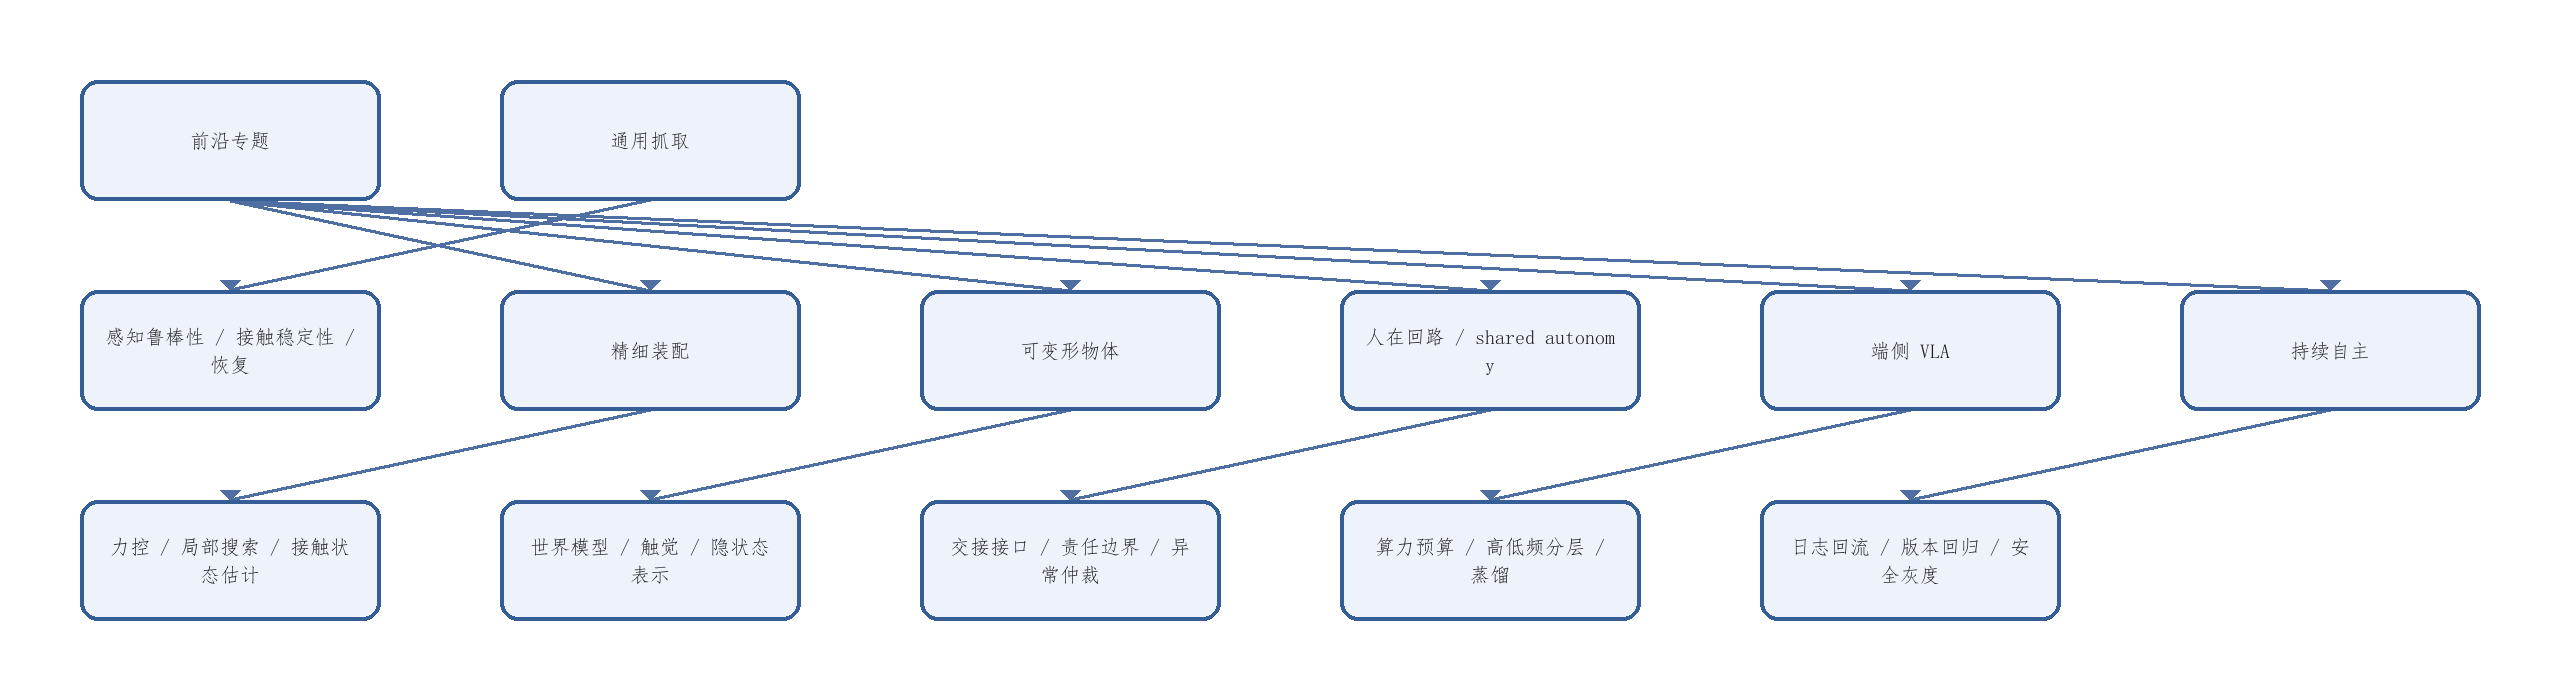
\includegraphics[width=0.9\textwidth,height=0.72\textheight,keepaspectratio]{figures/17-前沿专题与系统瓶颈图.png}
\caption{17-前沿专题与系统瓶颈图}
\label{fig:17-前沿专题与系统瓶颈图}
\end{figure}

\section*{专题映射补充}
\addcontentsline{toc}{chapter}{专题映射补充}
\markboth{专题映射补充}{专题映射补充}

本章最适合正式补成一张“前沿专题与对应系统瓶颈”映射表。它应明确指出：通用抓取主要考验感知与接触稳定性，精细装配主要考验力控与局部搜索，软体操作主要考验世界建模与触觉，端侧 VLA 主要考验算力与分层架构，持续自主则主要考验数据回流与验证基础设施。

这样做的好处是，前沿专题就不再只是热门方向清单，而会真正成为全书技术主干上的“难点坐标图”。

\section*{表 17-1 前沿专题与对应系统瓶颈映射表}
\addcontentsline{toc}{chapter}{表 17-1 前沿专题与对应系统瓶颈映射表}
\markboth{表 17-1 前沿专题与对应系统瓶颈映射表}{表 17-1 前沿专题与对应系统瓶颈映射表}

\begingroup
\small
\begin{xltabular}{\textwidth}{YYYY}
\toprule
前沿专题 & 主要瞄准的系统瓶颈 & 为什么它重要 & 当前典型难点 \\
\midrule
\endfirsthead
\toprule
前沿专题 & 主要瞄准的系统瓶颈 & 为什么它重要 & 当前典型难点 \\
\midrule
\endhead
通用抓取 & 感知-接触-恢复之间的闭环稳定性 & 是多数复杂操作能力的最小入口 & 遮挡、材质变化、抓取后滑移与重抓 \\
精细装配 & 局部搜索、力控、接触状态估计 & 能最直接暴露“会做任务”与“能稳定做成任务”的差距 & 公差小、力位协同难、失败代价高 \\
可变形物体操作 & 高维状态表示与接触预测 & 迫使系统超越刚体近似 & 状态难定义、视觉不足、接触后果复杂 \\
双臂与多指协同 & 多执行器协调与任务分工 & 接近真实复杂作业的必要前提 & 时序协调、空间互扰、接触分配 \\
端侧 VLA & 算力预算与高低频分层组织 & 决定高层模型是否能进入真实部署链路 & 延迟、热设计、模型压缩与异步调度 \\
持续自主 & 数据回流、版本回归与安全更新 & 决定系统是否能越用越强而非越改越乱 & 样本筛选、自动标注、灰度发布与回滚 \\
人在回路 / shared autonomy & 高风险场景下的责任与价值闭环 & 是许多现实行业先落地的组织形态 & 接管边界、界面设计、责任划分与 SLA \\
\bottomrule
\end{xltabular}
\endgroup
